\chapter{Introduction}\label{chap:introduction}

Inertial Sensor Units (IMU's) have become an everyday sensor in all kinds of devices, ranging from smart phones, drones, ships, autonomous cars or virtual reality headsets among others. 
One of the main reasons for that, is that they are conveniently complementary to the information that cameras capture, which are commonly found too in these devices. 
While the latter provide exteroceptive information about appearance and geometry up to scale, IMU's are proprioceptive sensors that make the previously unknown metric scale observable \cite{DBLP:journals/corr/ForsterCDS15}. 
Other reasons for their extended use are also their low power consumption, or the fact that they work even in darkness, or in GPS-denied environments \cite{DBLP:journals/corr/abs-1712-09004}.

However, either because of weight, space or economic constraints, most times the IMU's employed in these applications must be reduced in scale. 
Nowadays, \emph{Micro-electro-mechanical systems} (MEMS) have enabled to manufacture small and cheap enough IMU's, but these attributes come at the expense of higher sensor noise \cite{DBLP:journals/corr/abs-1802-02209}. 
Even if such noise is small, this renders traditional IMU integration unreliable as an Odometry method, as small errors in orientation lead to the so-called \emph{gravity leak} problem.
This phenomenon acts as a positive-feedback source of noise in position estimation, which in its turn results in a rapidly increasing drift of the estimation from the correct value \cite{Woodman07anintroduction}. 

Currently, there's a large variety of techniques that aim at leveraging other data input sources like cameras, or constraints/priors as for instance planar 2D motion, to cope with the IMU drift. 
Even so, the problem of Odometry in agile aerial robots (a 3D problem setup) remains a largely unsolved problem, and especially in the case of standalone Inertial Odometry (IO) \cite{DuoVIO}. 

On the other hand, Machine Learning (ML) and in particular Deep Learning (DL), have undergone a significant expansion in the last 10 years since the publication of AlexNet in 2012. 
In fact, recent approaches at odometry pipelines already include DL models to help solve this problem \cite{DBLP:journals/corr/abs-1802-02209, DBLP:journals/corr/ClarkWWMT17, DBLP:journals/corr/abs-1803-05850}.

In this thesis, we aim at progressing the research of Inertial navigation using a DL strategy. 
We will be combining ideas from several state-of-the-art publications into three IO-related state estimation pipelines, and analyzing their results. 
Because of that, in this work we will step away from any leveraging technique that uses inertial measurements combined with any other source of state observations, and tackle the problem of IO right at its core.
Furthermore, we will be using 3D datasets recorded by aerial units, as this is the most challenging form of the problem we can encounter with aboundant training data, where for instance assumptions on planar motion are not valid.


\section{Related Work}\label{sec:related_work}

In this section we will be reviewing several recent publications that have proposed novel methods of working with inertial data with a deep learning setup. 
We will be paying special attention to the studies that tackle the specific problem of IO, but we will also be exploring other approaches of IMU processing using DL in a broader VIO pipeline.

\subsection{Convolutional Neural Networks for speed regression}\label{sec:speed_reg}
The first work that we want to discuss is a very recent effort by Cort\'es et.al.  \cite{DBLP:journals/corr/abs-1808-03485}, which in fact inspired this project. 
In their work, a Convolutional Neural Network (CNN) regressor is used to predict the speed (i.e. the average modulus of the velocity vector $\hat{s} = \left \| \mathbf{\hat{v}}\right \|$) over a window of time (see Figure \ref{fig:original_speed_net}) just from its IMU measurements. 
The datasets used in this study are recorded by several people with a smartphone, making different walking patterns.
Their objective is to use the calculated speed values provided by the CNN model in a nonlinear state estimation pipeline, to track the position of the user over time. 

\begin{figure}[h]
   \centering
   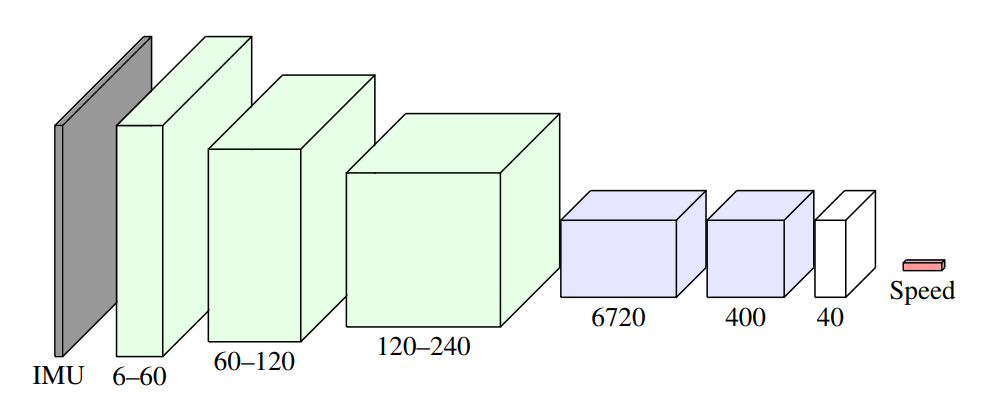
\includegraphics[width=0.75\textwidth]{thesis_template/img/cortes_cnn_architecture.png}
   \caption{CNN architecture from \cite{DBLP:journals/corr/abs-1808-03485}. This model is trained to estimate the speed norm of a moving object from a windowed sequence of IMU data. 
   Green layers are convolutional and the rest are fully connected (white does not have activation).}
   \label{fig:original_speed_net}
\end{figure}


In particular, the CNN model $f_\theta(\cdot)$ parametrized by $\theta$ estimates $\hat{s}$ using a $w\times6$ array of IMU data. 
Here \emph{w} is am hyper-parameter describing the number of IMU samples used as input, and 6 refers to the 6 Degree-of-Freedoms (DoF) of data captured by the IMU. 
In this case and during the rest of this report, IMU data will be assumed of 6 DoF (3 for gyroscope and 3 for accelerometer).
In other words, the model performs the computation described by \ref{eq:cnn_speed_regression}: 
\begin{equation}\label{eq:cnn_speed_regression}
    f_\theta\left(\mathbf{\hat{M}}_{k}\right) \rightarrow \hat{s}(k), \;\;\; \mathbf{\hat{M}}_{k}\in\mathbb{R}^{w\times6}, \;\hat{s}(k)=\left \| \mathbf{\hat{v}}(k)\right \|\in\mathbb{R}, \; \mathbf{\hat{v}}(k)\in\mathbb{R}^3.
\end{equation}
Where the variable \emph{k} refers to an arbitrary discrete time sample, such that $\mathbf{\hat{M}}_k$ comprises \emph{w} time samples between $\mathbf{\hat{M}}\!\left(k-w\right)$ and  $\mathbf{\hat{M}}\!\left(k\right)$. 
Indeed, $\mathbf{\hat{M}}$ includes both the information of the gyroscope and accelerometer, and has the structure given in \ref{eq:imu_img}.
\begin{equation}\label{eq:imu_img}
    \mathbf{\hat{M}}_k = \begin{bmatrix}
        _{B}\mathbf{\hat{a}}(k-w) & _{B}\mathbf{\hat{\boldsymbol{\omega}}}(k-w)\\ 
        _{B}\mathbf{\hat{a}}(k-w+1) & _{B}\mathbf{\hat{\boldsymbol{\omega}}}(k-w+1)\\ 
        \vdots & \vdots \\ 
        _{B}\mathbf{\hat{a}}(k) & _{B}\mathbf{\hat{\boldsymbol{\omega}}}(k)\\  
        \end{bmatrix} \in\mathbb{R}^{w\times6}.
\end{equation}
$\mathbf{\hat{M}}_k$ is composed by $_{B}\mathbf{\hat{a}}$ and $_{B}\mathbf{\hat{\boldsymbol{\omega}}}$, which are the observed acceleration and angular rates with the IMU respectively.
We will use the \emph{hat} ($\;\hat{}\;$) operator to indicate an estimated (or noisily observed) value, and \emph{k} and \emph{t} to refer to discrete and continuous time indices respectively from now on.
As a consequence, $\hat{s}(k)$ is the estimated \emph{average} speed during the time window between $(k-w, k)$. 
Such value predicted by the model is then fed as a low-confidence measurement update in an Extended Kalman Filter (EKF) pipeline \cite{DBLP:journals/corr/SolinCRK17}. 
For this particular study, the authors were using a 100Hz inertial sensor, and a two second window of data, i.e. $w = 200$.

The performance of their deep speed regressor is tested against a pedestrian dataset containing walking, static, stair climbing sequences, and achieves a RMSE error of $0.2\; m/s$.
Despite this, the performance of the model is worse than that for the stair sequences, which the authors justify as a lack of training samples of that particular type. 

\subsection{Recurrent Neural Networks for 2D IO}\label{sec:ionet}

This next work by Chen et.al. \cite{DBLP:journals/corr/abs-1802-02209} is somewhat more ambitious than the previous one, in the sense that it aims at performing end-to-end in-plane inertial odometry with, once again, walking datasets. 
In this planar setup, the agent state $\mathbf{x}$ can be defined by three degrees of freedom: two for position ($x$, $y$) and one for orientation/yaw ($\psi$). 
Similarly than before, the aim is to predict the state $\mathbf{x}(t+\Delta t)$ using only the IMU measurements belonging to the time window between $t$ and $t + \Delta t$.

However, as indicated by the authors of this paper, and interestingly unnoticed by the authors of \cite{DBLP:journals/corr/abs-1808-03485}, this problem setup is an ill-posed one.
This is because to predict the state $\mathbf{x}(t+\Delta t)$ the initial state $\mathbf{x}(t)$ is necessary, and therefore the IMU data alone is not enough for this task. 
Fortunately, the authors are able to demonstrate that by reformulating the problem into predicting the state increment $\Delta\mathbf{x} = (\Delta x, \Delta y, \Delta \psi)^{T}$, then the solution becomes independent of the initial state. 
In fact, it is possible to reduce the DoF of $\Delta\mathbf{x}$ further to only 2 by means of polar coordinates: $(\Delta l, \Delta \psi)^{T}$

In particular, as shown in \ref{eq:state_change_formulation}, the authors derive a formulation where the state increment $\Delta\mathbf{x}$ is a function of the initial velocity, gravity vector and IMU readings (all in body frame).
In theory, it is therefore possible to build a parametrized model $f_\theta$ such that it calculates the state shift from these inputs:
\begin{equation}\label{eq:state_change_formulation}
    f_\theta\left(_B\mathbf{g}(t), _{B}\mathbf{v}(t),_{B}\!\mathbf{\hat{a}}(t\!:\!t+\Delta t),_{B}\!\mathbf{\hat{\boldsymbol{\omega}}}(t\!:\!t+\Delta t)\right)\rightarrow\Delta\mathbf{x}, \;\;\;_{B}\mathbf{\hat{a}}, _{B}\!\mathbf{\hat{\boldsymbol{\omega}}}\in\mathbb{R}^3.
\end{equation}
Notice that the entire formulation works with 3D vectors, although the z position is assumed to be constant.
Furthermore, the authors argue that it is possible that the variables $\mathbf{g}(t)$ and $\mathbf{v}(t)$ are in fact latent variables of the sequence $\left(\mathbf{\hat{a}}(t\!:\!t+\Delta t),\mathbf{\hat{\boldsymbol{\omega}}}(t\!:\!t+\Delta t)\right)$, where the $B$ subindex has been dropped for readability. 

With this idea, the discrete time deep regressor would compute the estimated state increment as shown in \ref{eq:ionet_state_increment}.
\begin{equation}\label{eq:ionet_state_increment}
    f_\theta(\mathbf{\hat{M}}_{k}) \rightarrow \Delta\mathbf{\hat{x}}(k), \;\;\; \mathbf{\hat{M}}_{k}\in\mathbb{R}^{w\times6}, \;\Delta\mathbf{\hat{x}}(k)\in\mathbb{R}^{2}.
\end{equation}
Where again $\mathbf{\hat{M}}_{k}$ are the IMU measurements over a window of time equivalent to $\Delta t$. Finally, the estimated state increment $\Delta\mathbf{\hat{x}}=(\Delta \hat{l}, \Delta \hat{\psi})^{T}$, is used to compute $\mathbf{\hat{x}}(k+w)$ from $\mathbf{x}(k)$ as specified in \ref{eq:state_increment_2d}.
 \begin{equation}\label{eq:state_increment_2d}
     \mathbf{\hat{x}}(k+w)=\mathbf{x}(k) +
    \begin{bmatrix} 
    \Delta \hat{l}\cdot\cos\left(\psi(k)+\Delta\hat{\psi}\right) \\
    \Delta \hat{l}\cdot\sin\left(\psi(k)+\Delta\hat{\psi}\right) \\ 
    \Delta\hat{\psi} 
    \end{bmatrix}.
 \end{equation}

Another interesting point of this article is that, with the reasoning that IMU data has a strong temporal dependence over a window of time, Recurrent Neural Networks (RNN's) may be an interesting architecture to extract temporally correlated features out of it.
In particular, their expectation is that this kind of layer will be able to extract the missing latent variables $\mathbf{g}(t)$ and $\mathbf{v}(t)$ from the IMU measurements sequences, therefore rendering the problem completely independent of any variable except from $\mathbf{\hat{M}}_{k}$.
In particular, they use the Long Short-Term Memory (LSTM) architecture \cite{hochreiter1997long}, which has been shown to preserve better the gradients over time than its vanilla Recurrent layer counterpart \cite{DBLP:journals/corr/GreffSKSS15}. 

Their proposed deep model is actually quite simple, as it consists of simply two stacked LSTM layers (see Figure \ref{fig:original_ionet}). 
The first one creates a 96-dimensional hidden state (with ideally the latent variables), which serves as input to the second layer. 
The latter finally spits out a 2-dimensional value, corresponding to the polar state increment $\Delta\mathbf{\hat{x}}$. 
In fact, they empirically show that by using a \emph{bidirectional} LSTM layer (i.e. a layer that uses both past and future data to predict the displacement), the model gains slight benefits in training time compared to the non-bidirectional approach. 
Furthermore, they also train a CNN model for comparison purposes, which is shown to train considerably slower than the LSTM. 
Unfortunately, no further details about this CNN model architecture are provided.

\begin{figure}[h]
   \centering
   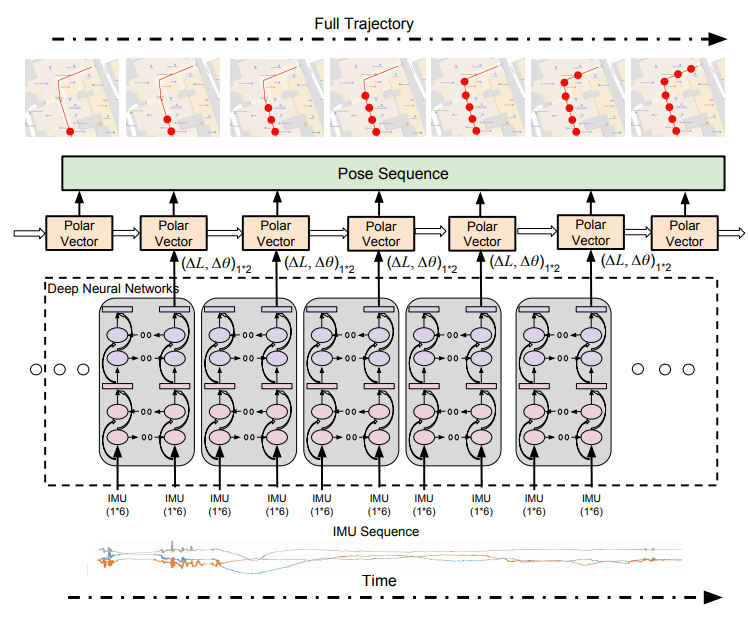
\includegraphics[width=0.75\textwidth]{thesis_template/img/ionet_original_architecture.png}
   \caption{RNN architecture from \cite{DBLP:journals/corr/abs-1802-02209} that predicts polar state increments in 2D (position + rotation) from IMU data. Two concatenated LSTM layers process the inertial input, and output a two component vector corresponding to the predicted the state increment $\Delta\mathbf{\hat{x}}$. This is later applied to the previous poses to generate a new pose in the sequence.}
   \label{fig:original_ionet}
\end{figure}
\subsection{Other usages of DL in Visual-Inertial Odometry}

The two previously introduced studies were thoroughly discussed as they both strictly fit in the use case of DL for IO (or closely related) purposes.  
However, there are other works that are worth mentioning in which DL is employed in the Visual-Inertial Odometry (VIO) problem. 

\subsubsection{Multirate CNN-RNN based VIO}\label{sec:VIOnet}
For instance, Clark and his team proposed in 2017 the idea of embedding a CNN network with an LSTM-based architecture in a VIO pipeline \cite{DBLP:journals/corr/ClarkWWMT17}. 
In particular, the convolutional layers are used to extract a low-rate feature vector from the optical flow between two image frames, and the recurrent ones to do the same at a higher rate with an IMU. 
Both outputs are then combined into a second (core) LSTM model that generates, similarly to \cite{DBLP:journals/corr/abs-1802-02209}, a state increment $\Delta\mathbf{\hat{x}}$.
Such increment prediction is then concatenated with the previous state estimate, and fed back to the core LSTM. The architecture schematic from the original publication is provided in Figure \ref{fig:original_vionet}. 

\begin{figure}[h]
   \centering
   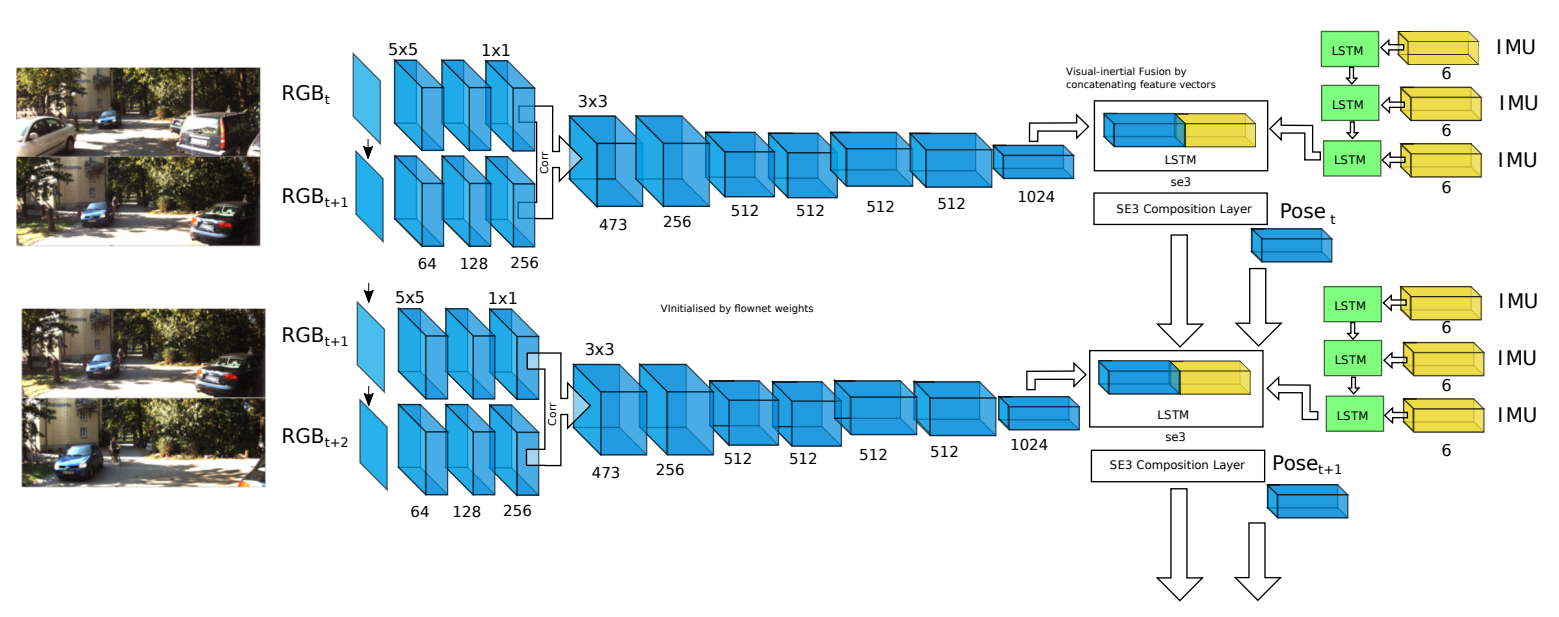
\includegraphics[width=0.90\textwidth]{thesis_template/img/vionet_original_architecture.png}
   \caption{CNN-RNN architecture from \cite{DBLP:journals/corr/ClarkWWMT17} for VIO. A CNN sequentially processes the image frames, while an LSTM processes the IMU data. Both feature vectors are concatenated and fed to a second LSTM, which predicts the state increment. Since the IMU rate is higher than the image rate, the core LSTM is adjusted to handle this rate difference.}
   \label{fig:original_vionet}
\end{figure}

Although it is unclear how reliant this model is to its Inertial part compared to the visual part, their proposed method achieves a performance close to the OK-VIS algorithm \cite{okvis} in the EuRoC \cite{Burri25012016} Micro-Aerial Vehicle (MAV) 3D dataset and in the outdoors autonomous driving KITTI dataset \cite{Geiger2012CVPR, Geiger2013IJRR}. 
Furthermore, it proves to be arguably more robust than OK-VIS in the situations where the extrinsic calibration between the IMU and the camera is not ideal. 

Last but not least, this paper is the first to our knowledge that introduces the idea of using the Lie algebra representation of the rotation group $SO(3)$ to help during the training of the deep model.
More insights about this will be discussed in Section \ref{sec:lie_algebra}.

\subsubsection{Unsupervised VIO with online error correction}
Another interesting although a bit more divergent approach is described by Shamwell et. al. in \cite{DBLP:journals/corr/abs-1803-05850}. 
This time, the VIO problem is faced from the unsupervised point of view, as they build a model that iteratively estimates and improves an affine transformation matrix that maps an input image at time $t$ to a target image at time $t+\Delta t$.
Indeed, it is assumed that some transformation has occurred during $\Delta t$, such that the images are slightly unaligned.
Note that with this strategy, no need for ground truth is needed.

Using the same notation as with the previous equations, the optimization starts by a CNN model $f_\theta(\cdot)$ extracting features from a window of IMU samples $\mathbf{\hat{M}}_k$ ranging from time $k-w$ until $k$. 
The same convolutional network also outputs the six degrees of freedom $\hat{\boldsymbol{\theta}}_0(k)\!\in\mathbb{R}^6$ of an affine transformation matrix, where the subindex $0$ indicates that this is the first iteration of the refinement).
\begin{equation}
    f_\theta\left(\mathbf{\hat{M}}_{k}\right) \rightarrow \hat{\boldsymbol{\theta}}_0(k), \;\;\; \mathbf{\hat{M}}_{k}\in\mathbb{R}^{w\times6}, \;\hat{\boldsymbol{\theta}}_0(k)\in\mathbb{R}^6
\end{equation}
Then, $\hat{\boldsymbol{\theta}}_0(k)$ is used to warp the input image $\mathbf{I}(k-w)$, producing an estimate image $\mathbf{\hat{I}}_0(k)$, which differs pixel-wise from the target image at the end of the window $\mathbf{I}(k)$ by $\mathbf{E}_0(k)$.
The jacobian matrix $\mathbf{J}_0$ of the error with respect to the initial state $\mathbf{x}(k-w)$ given by \ref{eq:reprojection_jacobian} is computed, and fed back as input for a second CNN, which modifies the original $\hat{\boldsymbol{\theta}}_0(k)$ into $\hat{\boldsymbol{\theta}}_1(k)$.
\begin{equation}\label{eq:reprojection_jacobian}
    \mathbf{J}_0 = \frac{\partial \mathbf{E}_0(k)}{\partial \mathbf{x}(k-w)}=\frac{\partial\!\left( \mathbf{I}(k)-\mathbf{\hat{I}}_0(k)\right)}{\partial \mathbf{x}(k-w)}
\end{equation}
This cycle is iterated $m$ times, until the error for all iterations is minimized $\mathbf{E}_i(k), \;\forall i\in\{0,...,m-1\}$.
The architecture for the first unit of this network, which is the one relevant for our task (i.e. the one that processes the IMU data), is provided in Figure \ref{fig:first_unit_unsupervised_vio}.
For further information, the reader is referred to the original paper. 

\begin{figure}[h]
   \centering
   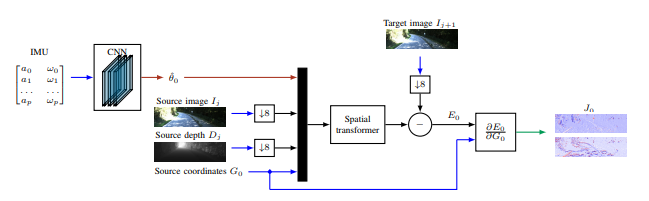
\includegraphics[width=0.90\textwidth]{thesis_template/img/unsupervised_VIO.png}
   \caption{Architecture for the first processing unit from \cite{DBLP:journals/corr/abs-1803-05850}. This unit receives the windowed IMU data as input and using a CNN outputs an affine transformation matrix estimate. 
   This transformation is applied to the initial image frame and subtracted pixel-wise from the next image frame.
   Finally, the jacobian matrix of the pixel difference derivative with respect to the initial state is computed, and fed to the next unit of this prediction system (not included in this figure).}
   \label{fig:first_unit_unsupervised_vio}
\end{figure}